
\clearpage
\newpage

\section{Post Experiments}

We provide a short description of newer experimental runs. 

\paragraph{Experimental Notes:} In the experiments 
we also used four nodes ({\tt sodb8}, {\tt sodb9}, {\tt sodb10}, and {\tt sodb12} ) in the same cluster. 
A short summary of the experiments is shown in Table~\ref{tab:exp_notes2}.

%% done
\begin{table}[h]
\begin{center}
\begin{tabular}{|p{4cm}|p{3cm}|p{4cm}|p{4cm}|} \hline
Machine & Task Length & Description & Time Length\\ \hline
{\tt sodb8} (plugged into \hbox{bottom} {\em left} power strip) &  INC16, INC13, and INC17.2 & Runs of 1,000 samples & 2018-03-17 $\sim$2018-03-18\\ \hline
{\tt sodb9}  (plugged into \hbox{bottom} {\em left} power strip)  &  IINC16, INC13, and INC17.2 & Runs of 1,000 samples & 2018-03-17 $\sim$2018-03-18\\ \hline
{\tt sodb10}  (plugged into \hbox{bottom} {\em left} power strip)  & INC16, INC13, and INC17.2 & Runs of 1,000 samples & 2018-03-17 $\sim$2018-03-18\\ \hline
{\tt sodb12}  (plugged into \hbox{bottom} {\em left} power strip)  & INC16, INC13, and INC17.2 & Runs of 1,000 samples & 2018-03-17 $\sim$2018-03-18\\ \hline
\end{tabular}
\end{center}
\vspace{-.2in}
\caption{Detailed description of INC data used for histograms\label{tab:exp_notes2}}
\end{table}

\subsection{Inter-Machine Homogeneity~\label{sec:diff_machine}} 

In this section we check if the use of different machines affects the distribution of execution (process) times on the same program. 
In other words, we examine {\em inter-machine repeatability}. For this examination, we use a nested for loop program, here termed INC, 
with different task lengths: 16 seconds, 13 seconds, and 17.2 seconds, each termed {\em INC16}, {\em INC13}, and {\em INC17.2}, respectively. 

Figures~\ref{fig:dm_1}, ~\ref{fig:dm_2}, and ~\ref{fig:dm_3} display the process time (PT) histograms on INC16, INC13, and INC17.2 run on our machines (from {\tt sodb8} to {\tt sodb12}), respectively. Based on these figures, we conclude that we should stick to one machine  for consistency, and {\tt sodb9} should be chosen in a sense that the data measured there consistently reveals a distinct binormal pattern.

\begin{figure}[h]
	\centering
	\subfigure[PT frequency on INC16]{
		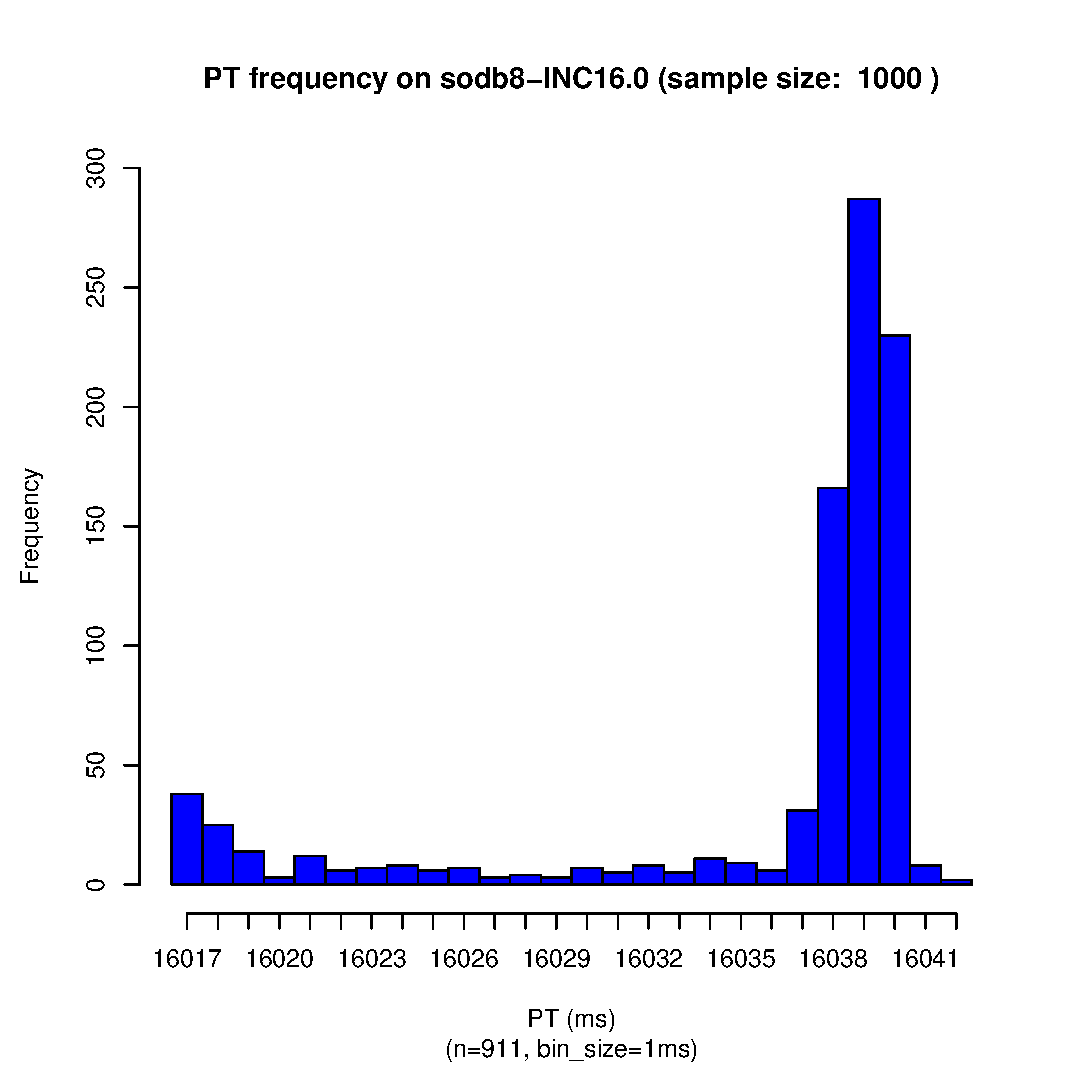
\includegraphics[scale=0.43]{newer_exp/sodb8_INC16_0_dist.eps}
		\label{fig:s8_inc16_dist}
	}	
	\subfigure[PT frequency on INC16]{
		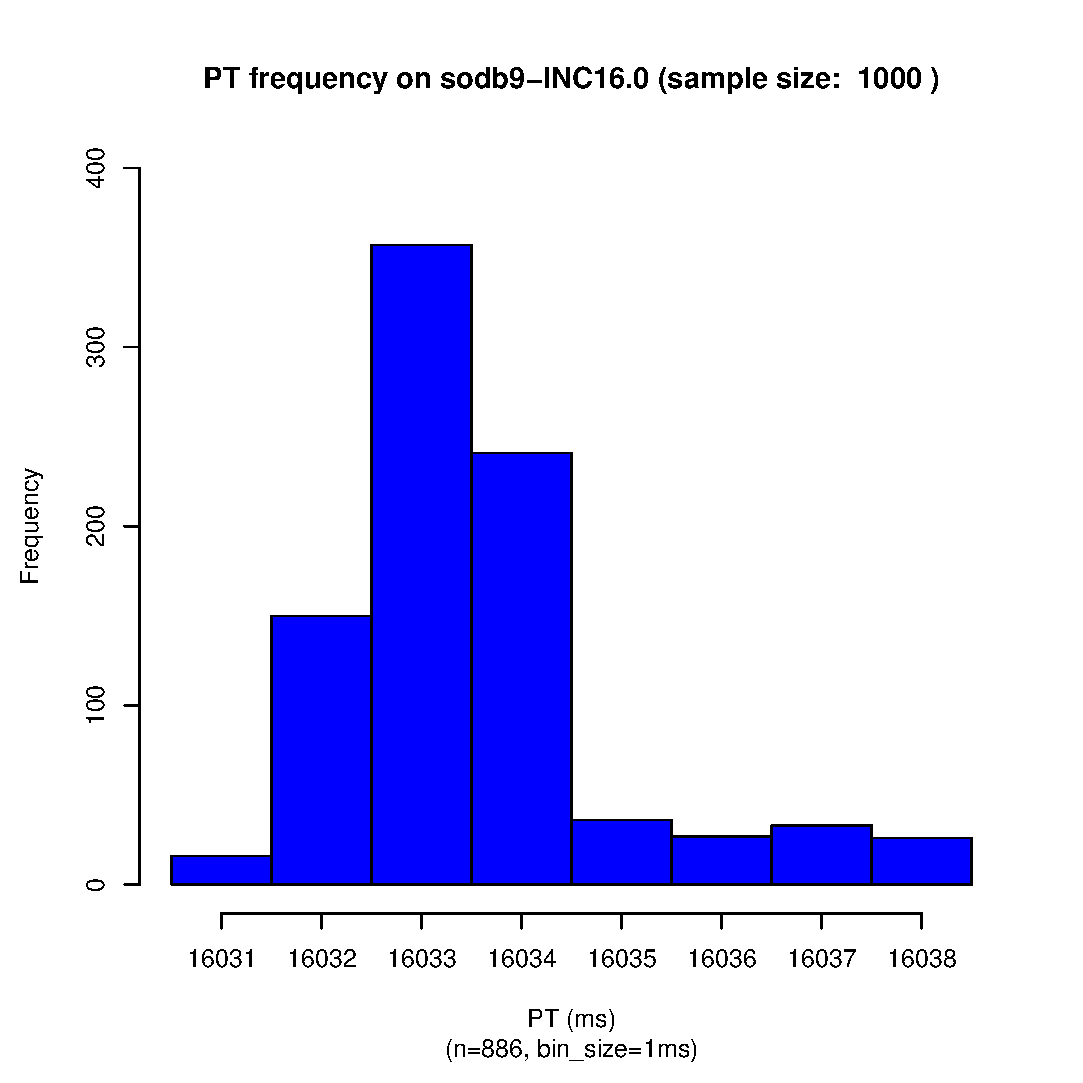
\includegraphics[scale=0.43]{newer_exp/sodb9_INC16_0_dist.eps}
		\label{fig:s9_inc16_dist}
	}
	\subfigure[PT frequency on INC16]{
		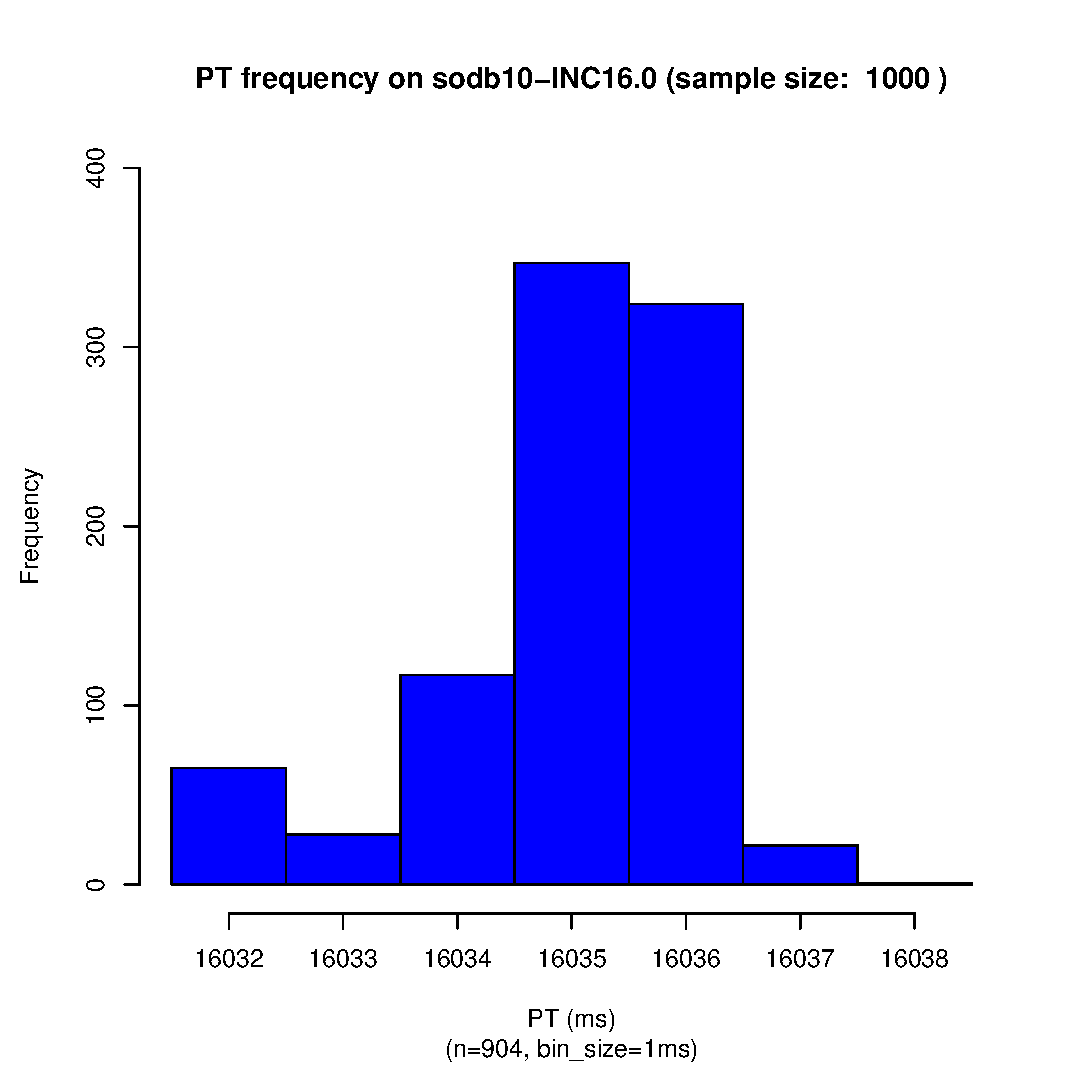
\includegraphics[scale=0.43]{newer_exp/sodb10_INC16_0_dist.eps}
		\label{fig:s10_inc16_dist}
	}	
	\subfigure[PT frequency on INC16]{
		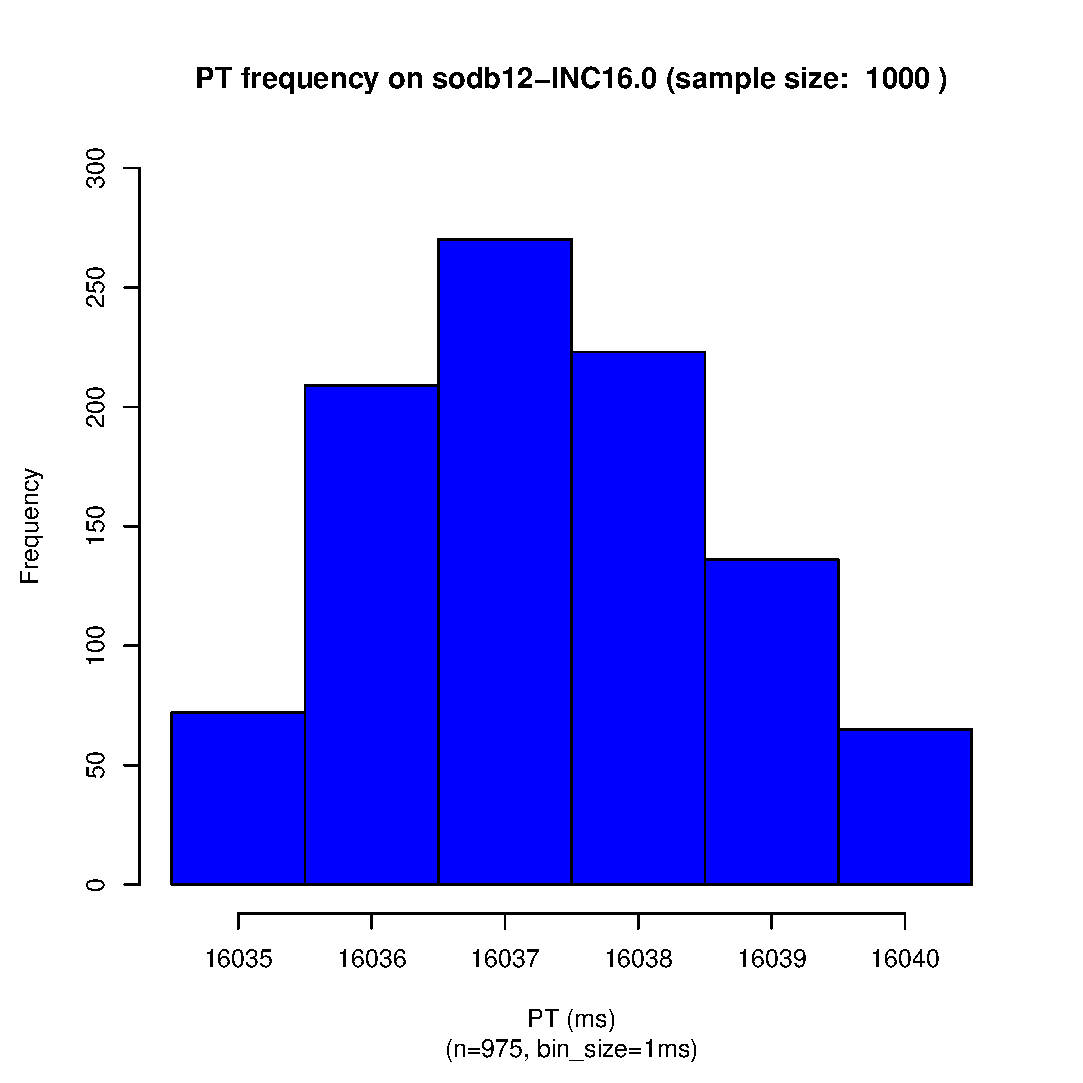
\includegraphics[scale=0.43]{newer_exp/sodb12_INC16_0_dist.eps}
		\label{fig:s12_inc16_dist}
	}
	\caption{PT Histograms on INC16~\label{fig:dm_1}}
\end{figure}


\newpage
\clearpage

\begin{figure}[h]
	\centering
	\subfigure[PT frequency on INC13]{
		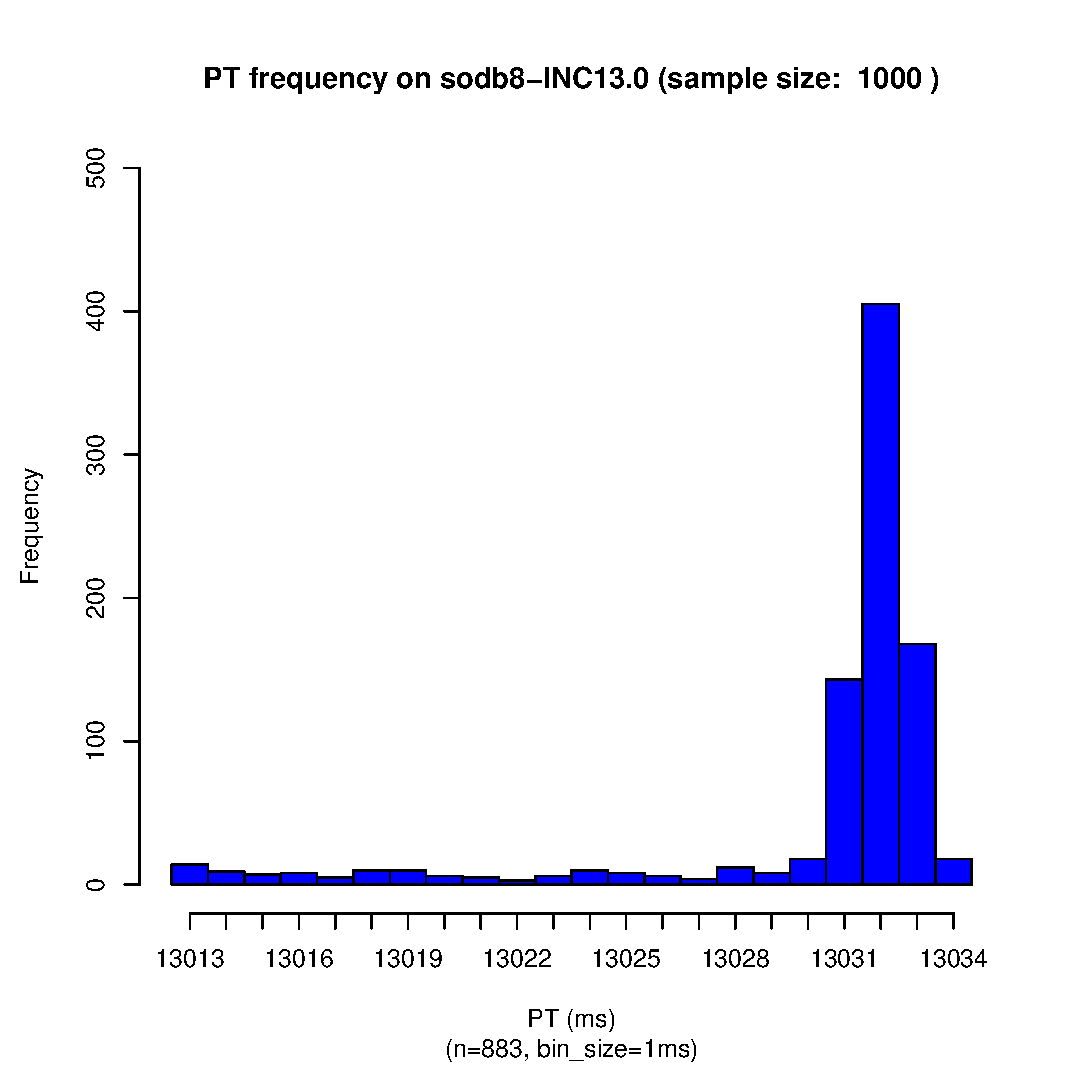
\includegraphics[scale=0.43]{newer_exp/sodb8_INC13_0_dist.eps}
		\label{fig:s8_inc13_dist}
	}	
	\subfigure[PT frequency on INC13]{
		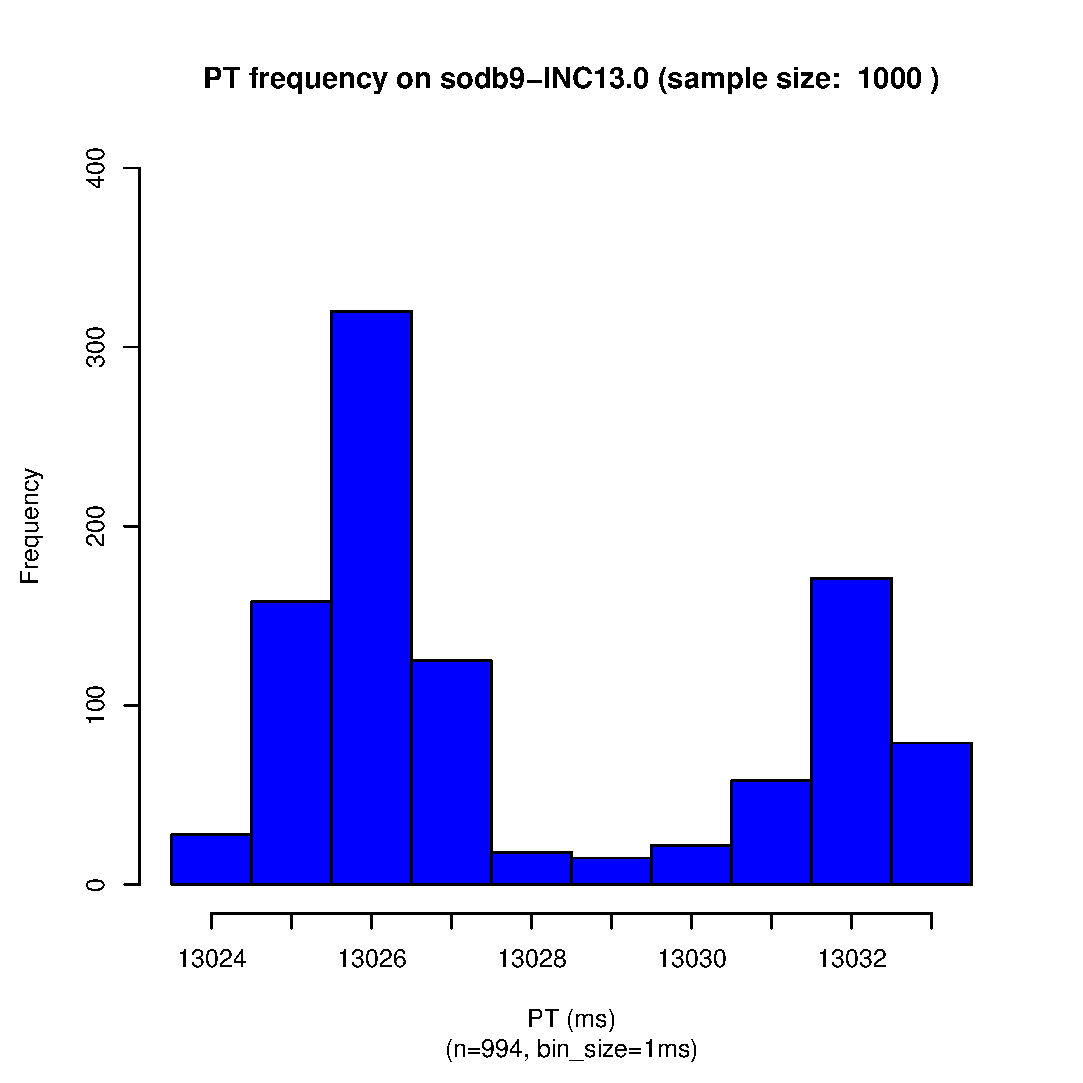
\includegraphics[scale=0.43]{newer_exp/sodb9_INC13_0_dist.eps}
		\label{fig:s9_inc13_dist}
	}
	\subfigure[PT frequency on INC13]{
		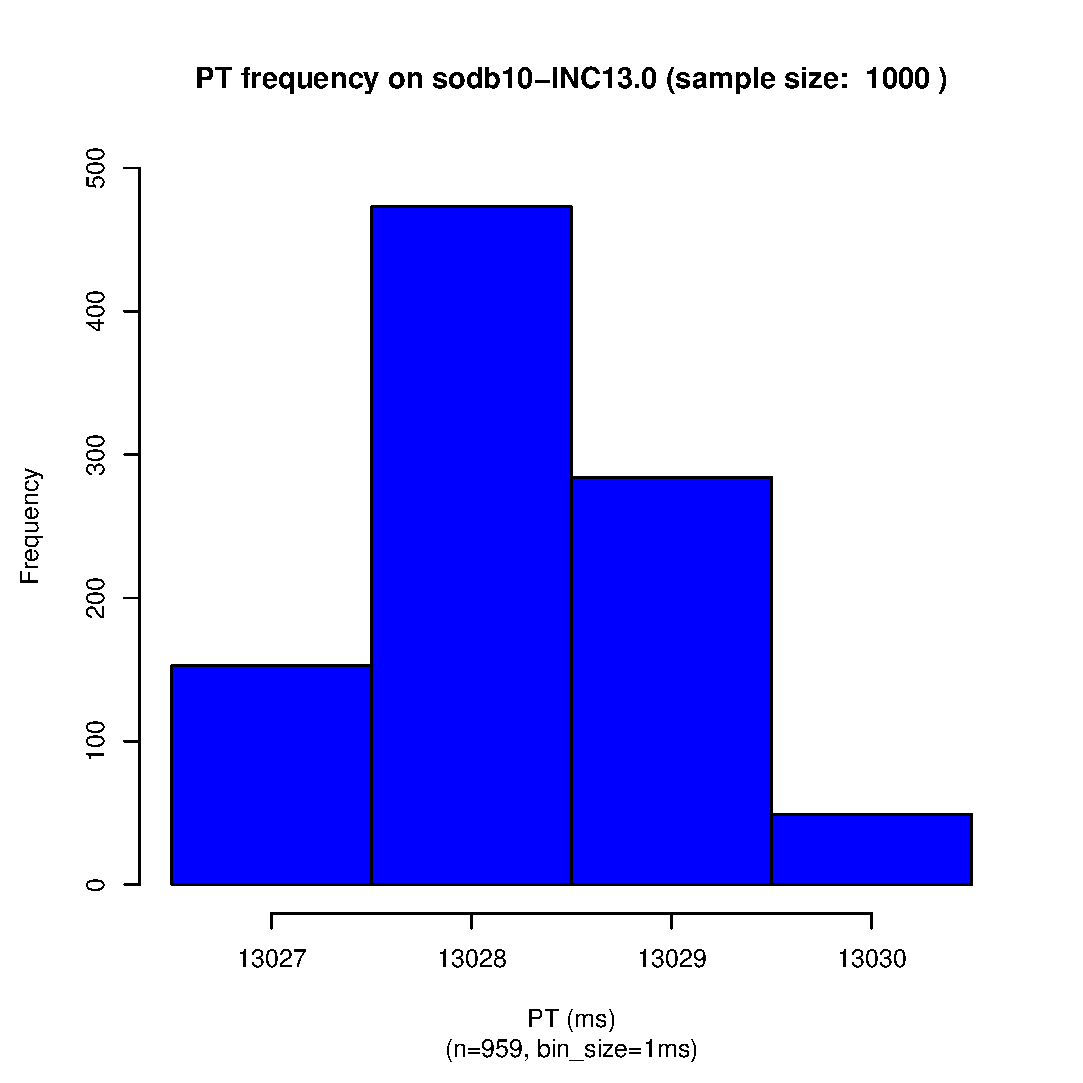
\includegraphics[scale=0.43]{newer_exp/sodb10_INC13_0_dist.eps}
		\label{fig:s10_inc13_dist}
	}	
	\subfigure[PT frequency on INC13]{
		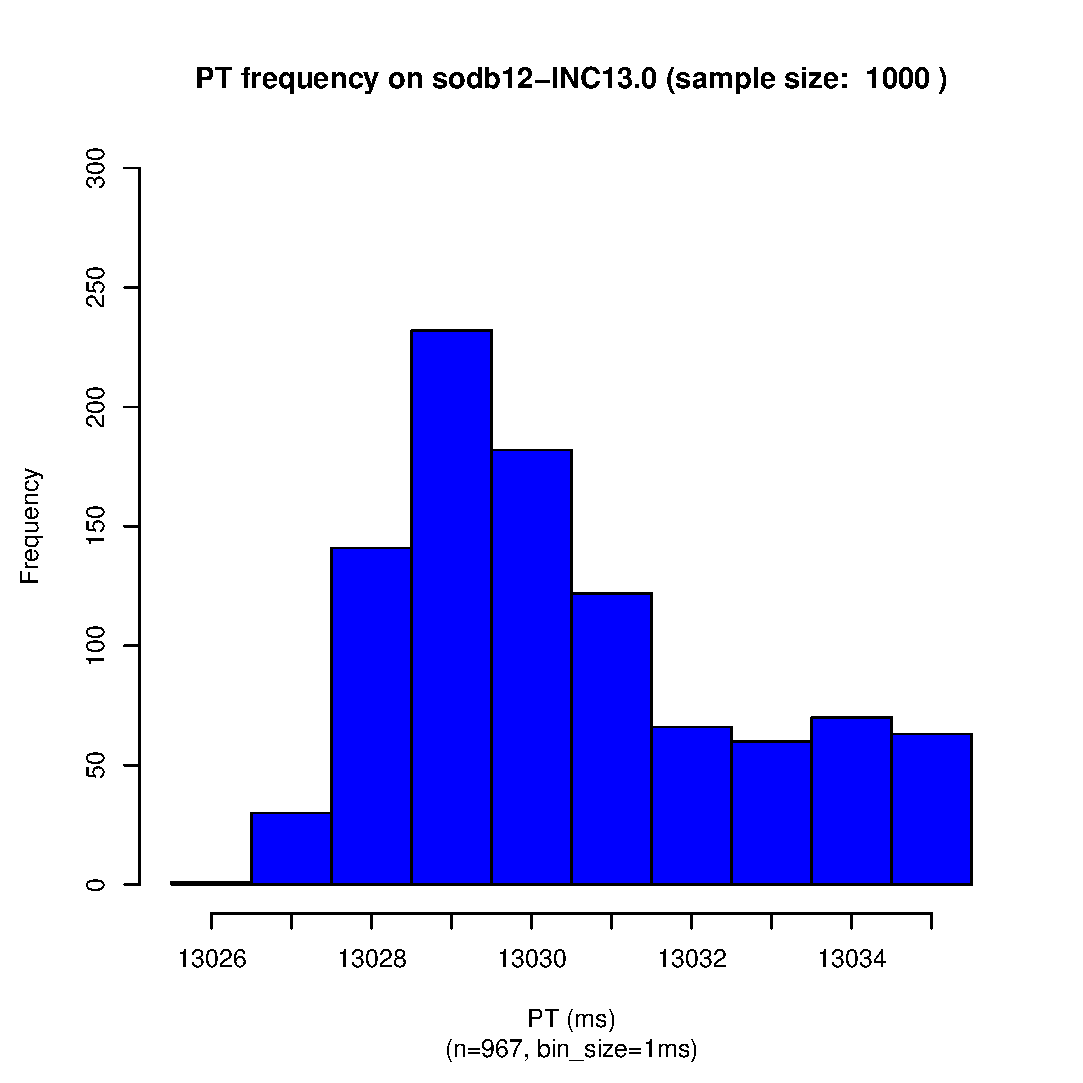
\includegraphics[scale=0.43]{newer_exp/sodb12_INC13_0_dist.eps}
		\label{fig:s12_inc13_dist}
	}
	\caption{PT Histograms on INC13~\label{fig:dm_2}}
\end{figure}

\newpage
\clearpage

\begin{figure}[h]
	\centering
	\subfigure[PT frequency on INC17.2]{
		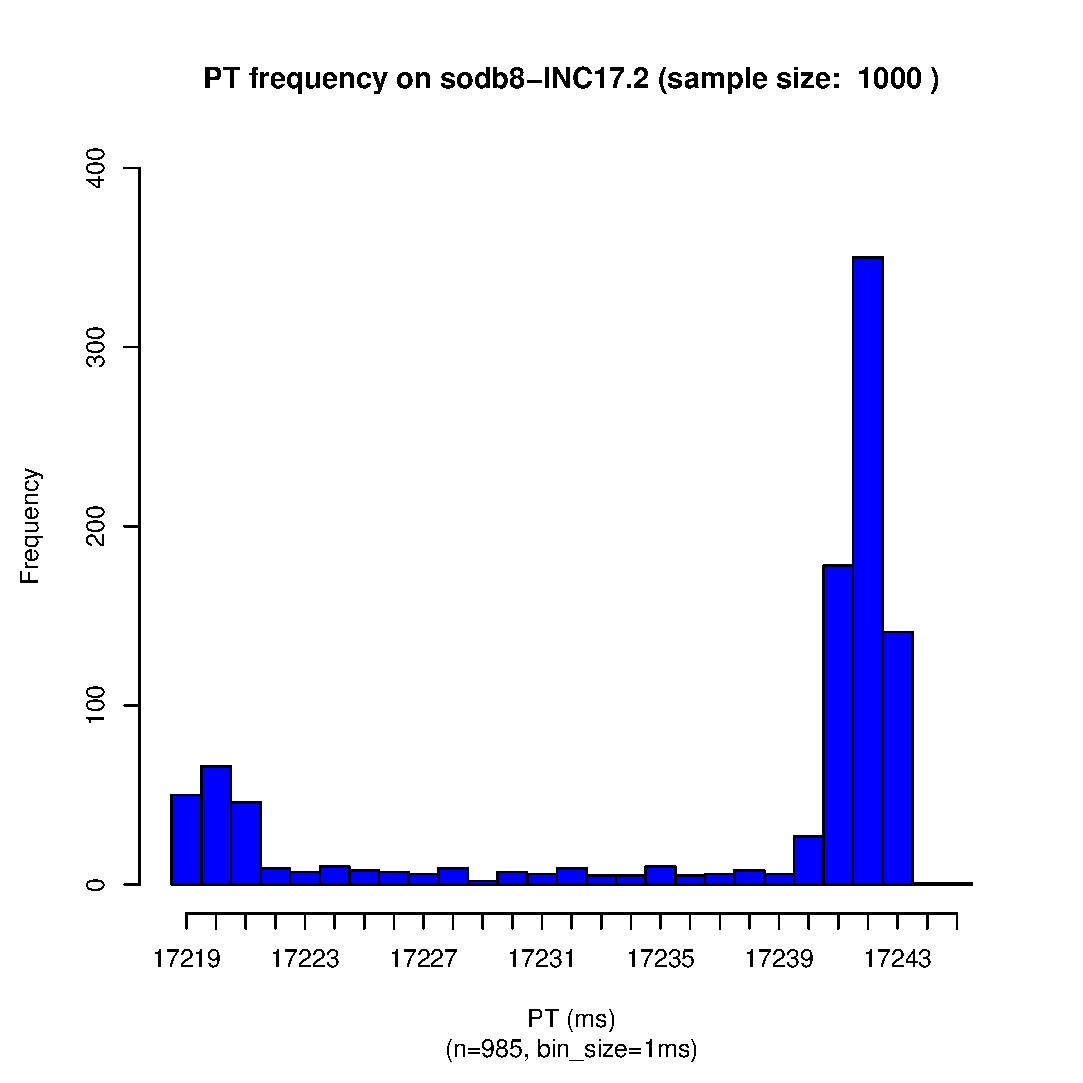
\includegraphics[scale=0.43]{newer_exp/sodb8_INC17_2_dist.eps}
		\label{fig:s8_inc17_2_dist}
	}	
	\subfigure[PT frequency on INC17.2]{
		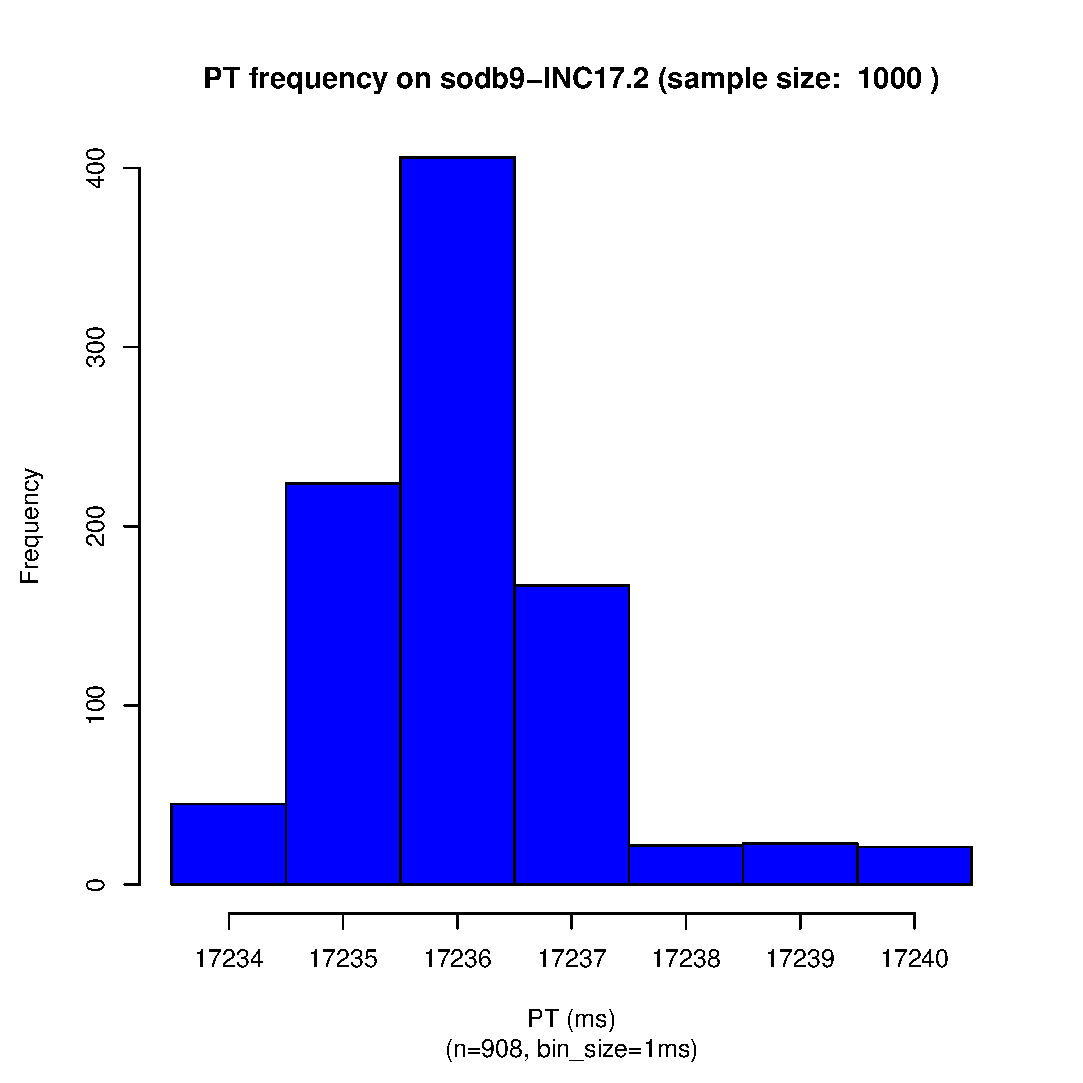
\includegraphics[scale=0.43]{newer_exp/sodb9_INC17_2_dist.eps}
		\label{fig:s9_inc17_2_dist}
	}
	\subfigure[PT frequency on INC17.2]{
		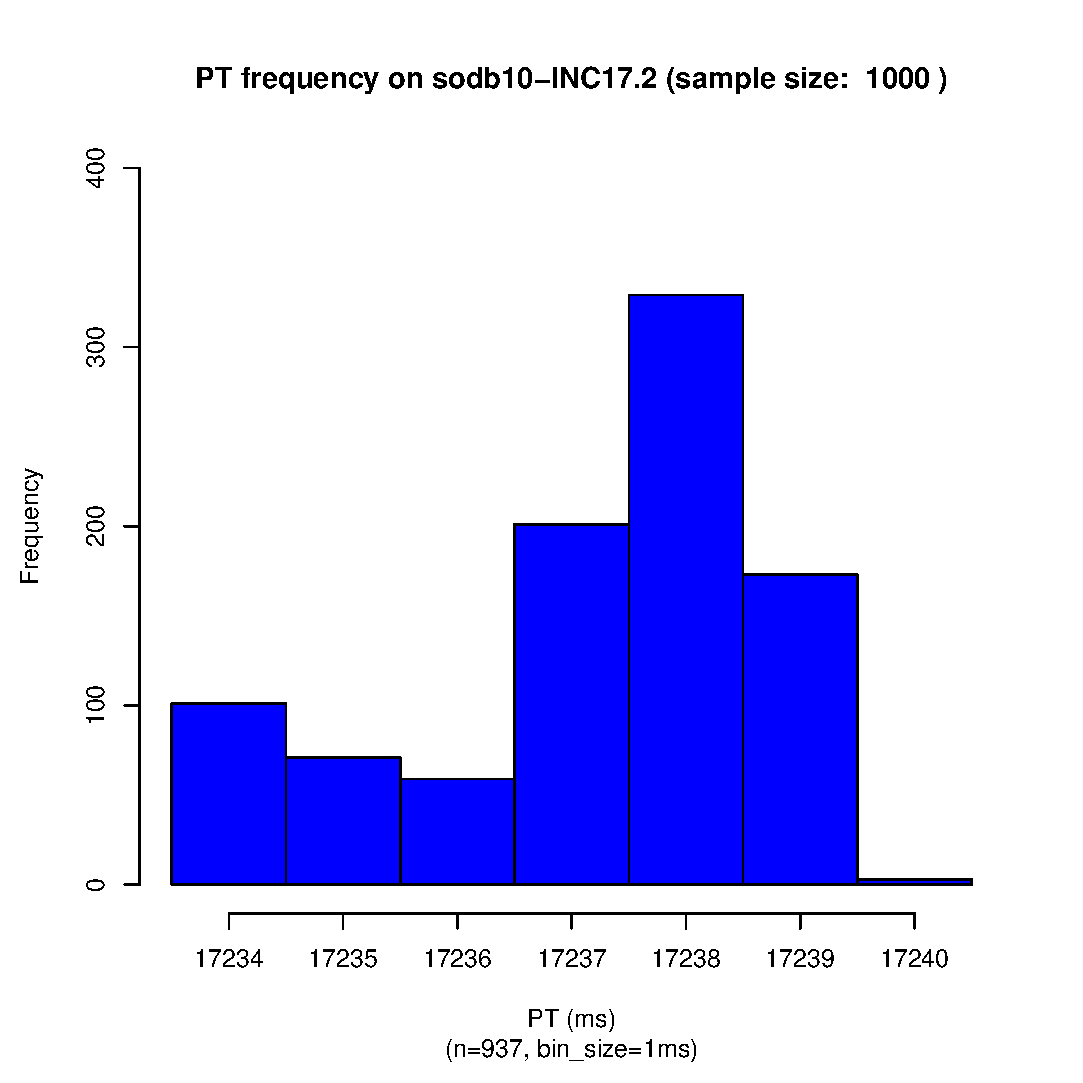
\includegraphics[scale=0.43]{newer_exp/sodb10_INC17_2_dist.eps}
		\label{fig:s10_inc17_2_dist}
	}	
	\subfigure[PT frequency on INC17.2]{
		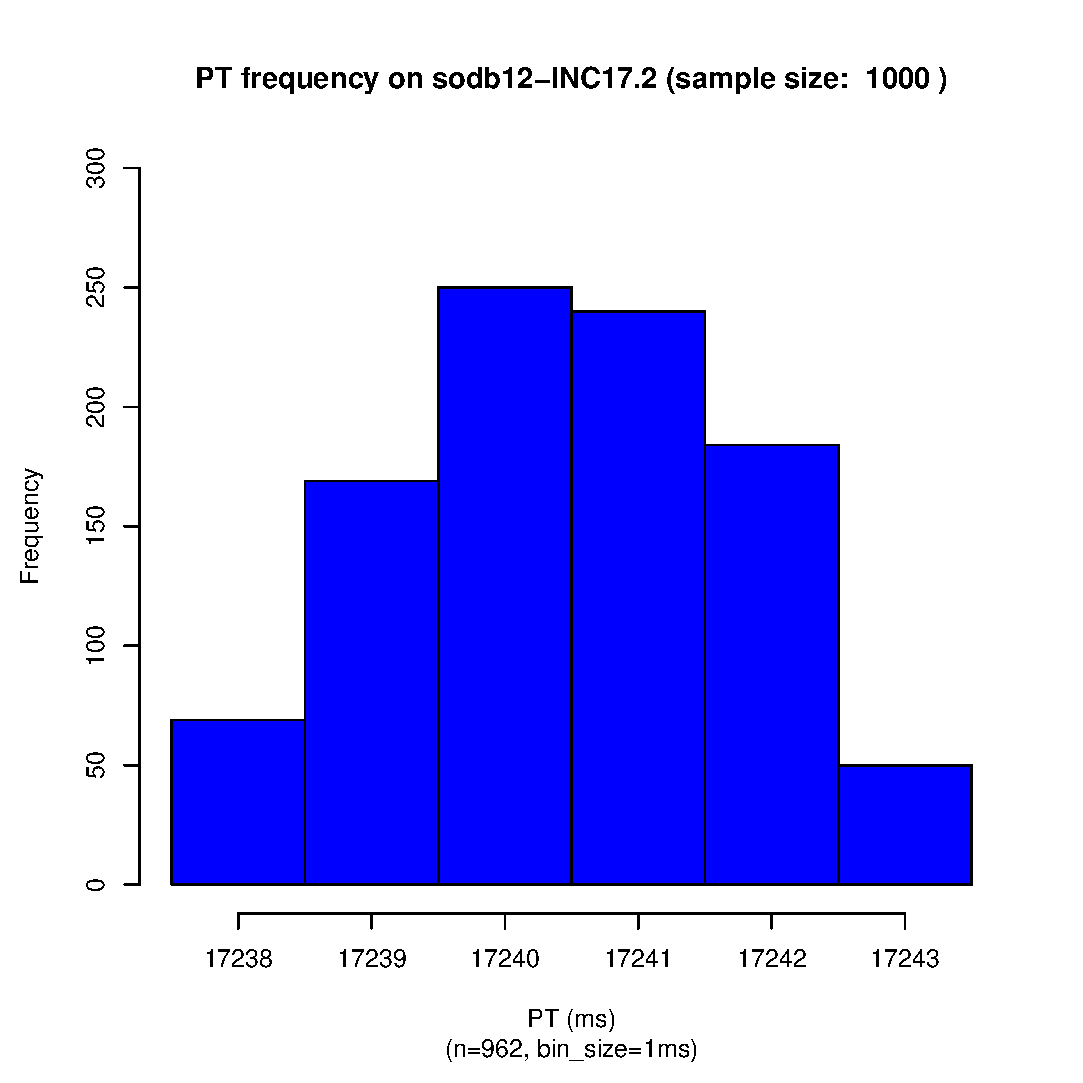
\includegraphics[scale=0.43]{newer_exp/sodb12_INC17_2_dist.eps}
		\label{fig:s12_inc17_2_dist}
	}
	\caption{PT Histograms on INC17.2~\label{fig:dm_3}}
\end{figure}

\newpage
\clearpage

\subsection{Investigation of Daemons' Influence on Program Time Distribution Regarding Machine Dependence~\label{sec:daemon_impact}} 

For the same task length, or INC16, 
I examined in each of the four runs a few iterations at which more than three daemons (except INC and proc monitor processes) that had positive PT were captured.  
From Table~\ref{fig:daemon}, I suspect that PT distribution seems most likely to be affected by two facts: {\it how longer the same daemon ran than usual}, and {\it how many different daemon processes appeared and how long it ran}.

\begin{table}[htp!]
\centering
{
 \begin{tabular}{|p{1.5cm}|p{2cm}|p{12.5cm}|} \hline
Machine Name & Iteration \# & Process Name (id, PT(msec))\\ \hline
{\tt sodb8}  & 174 & {\tt java} ({\tt 2349}, 15), {\tt java} ({\tt 2335}, 2),  {\tt md127\_raid1} ({\tt 457}, 1), {\tt kslowd000} ({\tt 166}, 1), {\tt kslowd001} ({\tt 167}, 1) \\ \cline{2-3}
 					& 278 & {\tt java} ({\tt 2877}, 16), {\tt java} ({\tt 2335}, 2),  {\tt kslowd000} ({\tt 166}, 1), {\tt kslowd001} ({\tt 167}, 1) \\ \cline{2-3}
			  &  486 & {\tt java} ({\tt 3190}, 21), {\tt java} ({\tt 2335}, 2),  {\tt md127\_raid1} ({\tt 457}, 1), {\tt kslowd000} ({\tt 166}, 1)\\ \cline{2-3}
				  &  526 & {\tt md127\_raid1} ({\tt 457}, 1), {\tt kslowd000} ({\tt 166}, 1), {\tt kslowd001} ({\tt 167}, 1), {\tt jbd2/md127-8} ({\tt 470}, 1)\\ \cline{2-3}
				  &  555 & {\tt java} ({\tt 3815}, 8), {\tt java} ({\tt 2335}, 2), {\tt kslowd000} ({\tt 166}, 1), {\tt kslowd001} ({\tt 167}, 1)\\ \hline
{\tt sodb9}  & 105 & {\tt java} ({\tt 6634}, 16), {\tt java} ({\tt 6621}, 2),  {\tt kslowd000} ({\tt 166}, 1), {\tt kslowd001} ({\tt 167}, 1) \\ \cline{2-3}
				  & 175 & {\tt java} ({\tt 6942}, 7), {\tt java} ({\tt 6621}, 2),  {\tt kslowd000} ({\tt 166}, 1), {\tt kslowd001} ({\tt 167}, 1) \\ \cline{2-3}
				  & 245 & {\tt java} ({\tt 7259}, 6), {\tt java} ({\tt 6621}, 2),  {\tt kslowd000} ({\tt 166}, 1), {\tt kslowd001} ({\tt 167}, 1) \\ \cline{2-3}
				  & 280 & {\tt java} ({\tt 7365}, 3), {\tt java} ({\tt 6621}, 2),  {\tt kslowd000} ({\tt 166}, 1), {\tt kslowd001} ({\tt 167}, 1) \\ \cline{2-3}
				  & 350 & {\tt java} ({\tt 7577}, 3), {\tt java} ({\tt 6621}, 2),  {\tt kslowd000} ({\tt 166}, 1), {\tt kslowd001} ({\tt 167}, 1) \\ \cline{2-3}
				  & 420 & {\tt java} ({\tt 7683}, 3), {\tt java} ({\tt 6621}, 2),  {\tt kslowd000} ({\tt 166}, 1), {\tt kslowd001} ({\tt 167}, 1) \\ \cline{2-3}
				  & 490 & {\tt java} ({\tt 7894}, 4), {\tt java} ({\tt 6621}, 2),  {\tt kslowd000} ({\tt 166}, 1), {\tt kslowd001} ({\tt 167}, 1) \\ \hline
{\tt sodb10}  & 105 & {\tt java} ({\tt 28394}, 14), {\tt java} ({\tt 28381}, 2),  {\tt kslowd000} ({\tt 166}, 1), {\tt kslowd001} ({\tt 167}, 1) \\ \cline{2-3}
					 & 314 & {\tt java} ({\tt 28702}, 18), {\tt java} ({\tt 28381}, 2),  {\tt md127\_raid1} ({\tt 455}, 1),  {\tt kslowd001} ({\tt 167}, 1) \\ \hline
 {\tt sodb12}  & 280 &  {\tt kslowd001} ({\tt 167}, 154),  {\tt kslowd000} ({\tt 166}, 150), {\tt java} ({\tt 14820}, 37), {\tt java} ({\tt 14807}, 2) \\ \cline{2-3}
	& 311 &  {\tt kslowd000} ({\tt 166}, 154),  {\tt kslowd001} ({\tt 167}, 153), {\tt java} ({\tt 14807}, 2), {\tt java} ({\tt 15653}, 1), {\tt khugepaged} ({\tt 30}, 1)\\ \cline{2-3}		& 373 &  {\tt kslowd000} ({\tt 166}, 154),  {\tt kslowd001} ({\tt 167}, 152), {\tt java} ({\tt 14807}, 2), {\tt java} ({\tt 15747}, 2)\\ \cline{2-3}
& 435 &  {\tt kslowd000} ({\tt 166}, 154),  {\tt kslowd001} ({\tt 167}, 153), {\tt java} ({\tt 15934}, 6), {\tt java} ({\tt 14807}, 2)\\ \cline{2-3}
& 466 &  {\tt kslowd000} ({\tt 166}, 152), {\tt java} ({\tt 16121}, 6), {\tt java} ({\tt 14807}, 2), {\tt kblockd/0} ({\tt 16}, 1)\\ \cline{2-3}
 \hline
 \end{tabular}
  }
 \caption{Some daemon processes captured across different machines~\label{fig:daemon}}
\end{table}